\documentclass[tikz,border=2mm]{standalone}
\usepackage{fix-cm}
\usepackage[scaled=0.92]{helvet}
\renewcommand{\familydefault}{\sfdefault}
\usepackage{tikz}
\usetikzlibrary{arrows.meta,calc,positioning,shapes.geometric}

\definecolor{blue}{HTML}{3B6EA8}
\definecolor{bluelight}{HTML}{EAF2F8}
\definecolor{teal}{HTML}{238C7E}
\definecolor{teallight}{HTML}{E8F5F2}
\definecolor{purple}{HTML}{755AA8}
\definecolor{purplelight}{HTML}{F1ECF8}
\definecolor{warm}{HTML}{C7653D}
\definecolor{warmlight}{HTML}{FAEEE8}
\definecolor{ink}{HTML}{24313D}
\definecolor{muted}{HTML}{5F6B75}
\definecolor{rule}{HTML}{B8C1C8}

\begin{document}
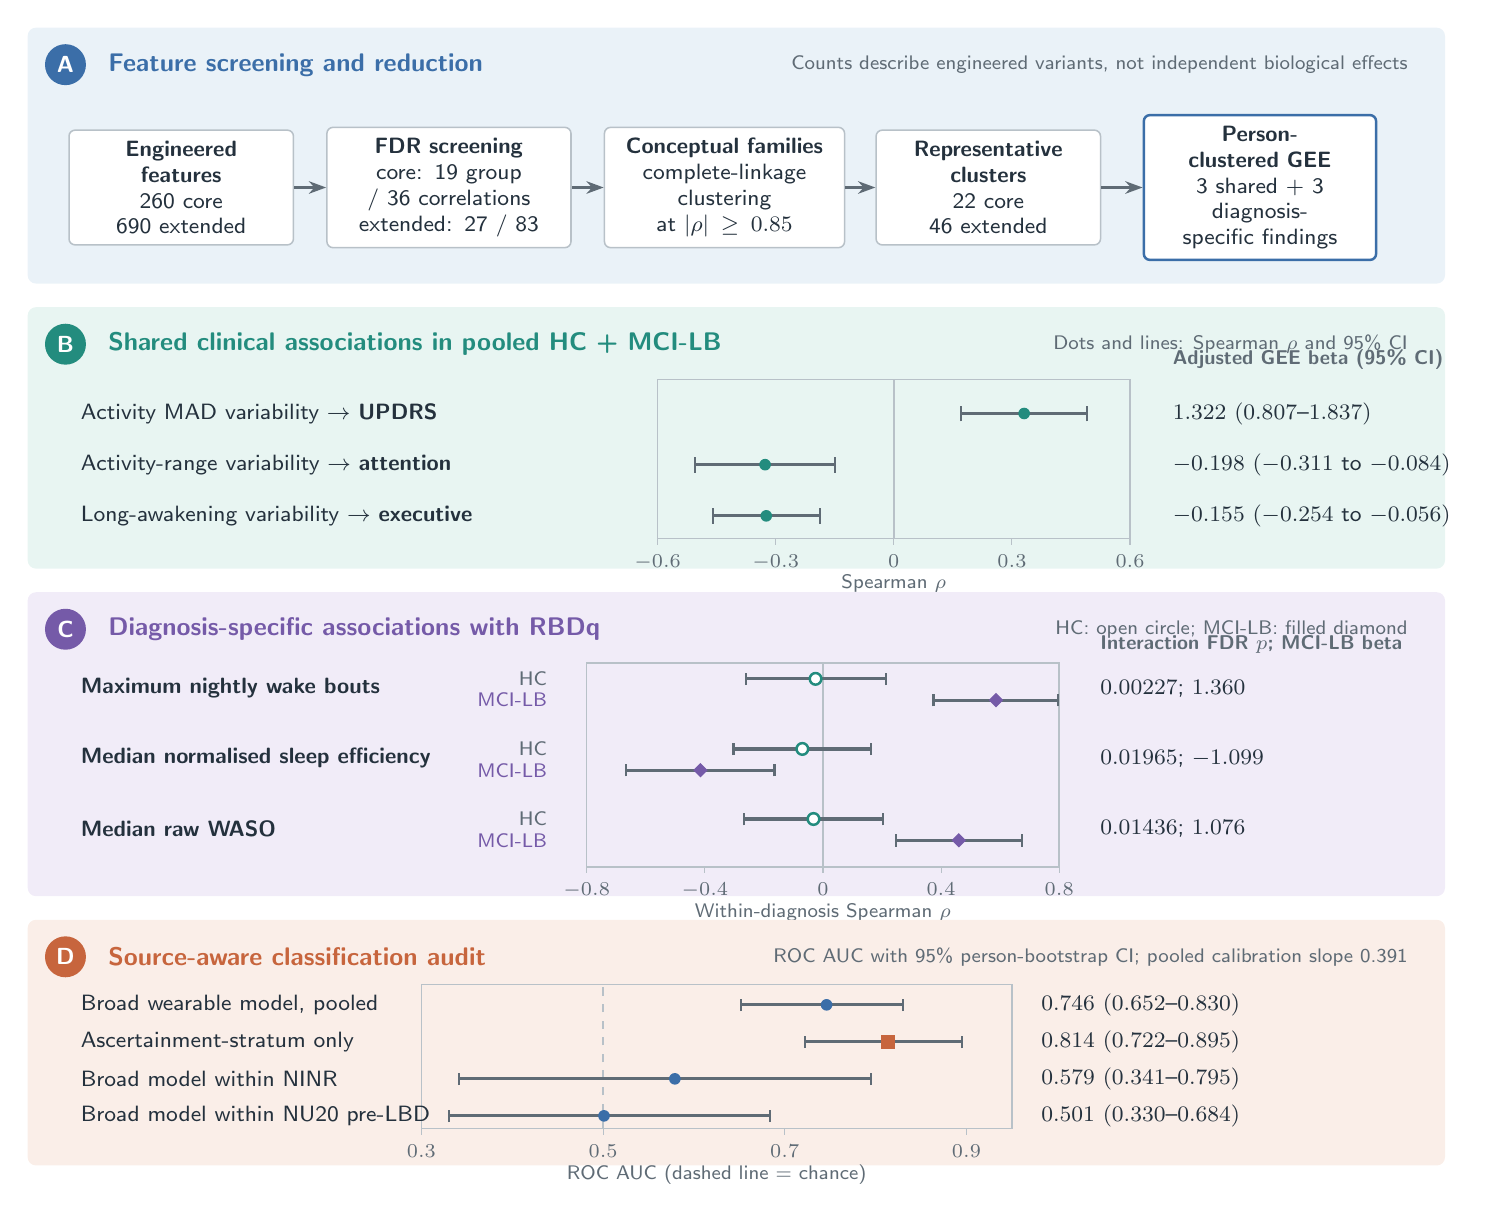
\begin{tikzpicture}[
  x=1cm,y=1cm,
  font=\fontsize{8.0}{9.3}\selectfont,
  text=ink,
  flow/.style={-{Stealth[length=2.2mm,width=1.6mm]}, line width=0.8pt, draw=muted},
  box/.style={draw=rule, line width=0.55pt, rounded corners=2.2pt,
    fill=white, align=center, inner sep=4pt, minimum height=1.25cm},
  paneltitle/.style={font=\bfseries\fontsize{9.2}{10.5}\selectfont, anchor=west},
  note/.style={font=\fontsize{7.1}{8.2}\selectfont, text=muted},
  tag/.style={circle, minimum size=5.2mm, inner sep=0pt, text=white,
    font=\bfseries\fontsize{8.4}{9}\selectfont},
  ci/.style={line width=1.15pt, draw=muted},
  cicap/.style={line width=0.8pt, draw=muted}
]

% Panel A: feature reduction
\fill[bluelight, rounded corners=3pt] (0,11.20) rectangle (18.0,14.45);
\node[tag, fill=blue] at (0.48,13.98) {A};
\node[paneltitle, text=blue] at (0.90,13.98) {Feature screening and reduction};
\node[note, anchor=east] at (17.65,13.98) {Counts describe engineered variants, not independent biological effects};

\node[box, minimum width=2.85cm, text width=2.48cm] (input) at (1.95,12.42)
  {\textbf{Engineered features}\\260 core\\690 extended};
\node[box, minimum width=3.10cm, text width=2.74cm] (screen) at (5.35,12.42)
  {\textbf{FDR screening}\\core: 19 group / 36 correlations\\extended: 27 / 83};
\node[box, minimum width=3.05cm, text width=2.68cm] (families) at (8.85,12.42)
  {\textbf{Conceptual families}\\complete-linkage clustering\\at $|\rho|\geq0.85$};
\node[box, minimum width=2.85cm, text width=2.48cm] (clusters) at (12.20,12.42)
  {\textbf{Representative clusters}\\22 core\\46 extended};
\node[box, minimum width=2.95cm, text width=2.58cm, draw=blue, line width=0.9pt] (followup) at (15.65,12.42)
  {\textbf{Person-clustered GEE}\\3 shared + 3 diagnosis-specific findings};
\draw[flow] (input.east) -- (screen.west);
\draw[flow] (screen.east) -- (families.west);
\draw[flow] (families.east) -- (clusters.west);
\draw[flow] (clusters.east) -- (followup.west);

% Panel B: shared associations
\fill[teallight, rounded corners=3pt] (0,7.58) rectangle (18.0,10.90);
\node[tag, fill=teal] at (0.48,10.43) {B};
\node[paneltitle, text=teal] at (0.90,10.43) {Shared clinical associations in pooled HC + MCI-LB};
\node[note, anchor=east] at (17.65,10.43) {Dots and lines: Spearman $\rho$ and 95\% CI};

% Forest frame and reference line
\draw[rule, line width=0.55pt] (8.00,7.96) rectangle (14.00,9.98);
\draw[rule, line width=0.65pt] (11.00,7.96) -- (11.00,9.98);
\foreach \x/\lab in {8.00/$-0.6$,9.50/$-0.3$,11.00/$0$,12.50/$0.3$,14.00/$0.6$}{
  \draw[rule] (\x,7.96) -- ++(0,-0.08);
  \node[note, anchor=north] at (\x,7.88) {\lab};
}
\node[note, anchor=north] at (11.00,7.62) {Spearman $\rho$};
\node[font=\bfseries\fontsize{7.2}{8.2}\selectfont, text=muted, anchor=south west] at (14.42,9.98)
  {Adjusted GEE beta (95\% CI)};

\node[anchor=west] at (0.55,9.55) {Activity MAD variability $\rightarrow$ \textbf{UPDRS}};
\draw[ci] (11.855,9.55) -- (13.450,9.55);
\draw[cicap] (11.855,9.45) -- (11.855,9.65);
\draw[cicap] (13.450,9.45) -- (13.450,9.65);
\fill[teal] (12.655,9.55) circle (2.1pt);
\node[anchor=west] at (14.42,9.55) {$1.322$ $(0.807$--$1.837)$};

\node[anchor=west] at (0.55,8.90) {Activity-range variability $\rightarrow$ \textbf{attention}};
\draw[ci] (8.470,8.90) -- (10.255,8.90);
\draw[cicap] (8.470,8.80) -- (8.470,9.00);
\draw[cicap] (10.255,8.80) -- (10.255,9.00);
\fill[teal] (9.365,8.90) circle (2.1pt);
\node[anchor=west] at (14.42,8.90) {$-0.198$ $(-0.311$ to $-0.084)$};

\node[anchor=west] at (0.55,8.25) {Long-awakening variability $\rightarrow$ \textbf{executive}};
\draw[ci] (8.705,8.25) -- (10.060,8.25);
\draw[cicap] (8.705,8.15) -- (8.705,8.35);
\draw[cicap] (10.060,8.15) -- (10.060,8.35);
\fill[teal] (9.380,8.25) circle (2.1pt);
\node[anchor=west] at (14.42,8.25) {$-0.155$ $(-0.254$ to $-0.056)$};

% Panel C: diagnosis-specific RBDq associations
\fill[purplelight, rounded corners=3pt] (0,3.42) rectangle (18.0,7.28);
\node[tag, fill=purple] at (0.48,6.81) {C};
\node[paneltitle, text=purple] at (0.90,6.81) {Diagnosis-specific associations with RBDq};
\node[note, anchor=east] at (17.65,6.81) {HC: open circle; MCI-LB: filled diamond};

\draw[rule, line width=0.55pt] (7.10,3.79) rectangle (13.10,6.38);
\draw[rule, line width=0.65pt] (10.10,3.79) -- (10.10,6.38);
\foreach \x/\lab in {7.10/$-0.8$,8.60/$-0.4$,10.10/$0$,11.60/$0.4$,13.10/$0.8$}{
  \draw[rule] (\x,3.79) -- ++(0,-0.08);
  \node[note, anchor=north] at (\x,3.71) {\lab};
}
\node[note, anchor=north] at (10.10,3.45) {Within-diagnosis Spearman $\rho$};
\node[font=\bfseries\fontsize{7.2}{8.2}\selectfont, text=muted, anchor=south west] at (13.50,6.38)
  {Interaction FDR $p$; MCI-LB beta};

\node[anchor=west] at (0.55,6.06) {\textbf{Maximum nightly wake bouts}};
\node[note, anchor=east] at (6.72,6.18) {HC};
\node[note, anchor=east, text=purple] at (6.72,5.91) {MCI-LB};
\draw[ci] (9.118,6.18) -- (10.899,6.18);
\draw[cicap] (9.118,6.10) -- (9.118,6.26); \draw[cicap] (10.899,6.10) -- (10.899,6.26);
\draw[teal, line width=0.9pt, fill=white] (10.006,6.18) circle (2.1pt);
\draw[ci] (11.503,5.91) -- (13.089,5.91);
\draw[cicap] (11.503,5.83) -- (11.503,5.99); \draw[cicap] (13.089,5.83) -- (13.089,5.99);
\node[diamond, fill=purple, draw=purple, minimum size=4.8pt, inner sep=0pt] at (12.298,5.91) {};
\node[anchor=west] at (13.50,6.05) {$0.00227$; $1.360$};

\node[anchor=west] at (0.55,5.17) {\textbf{Median normalised sleep efficiency}};
\node[note, anchor=east] at (6.72,5.29) {HC};
\node[note, anchor=east, text=purple] at (6.72,5.02) {MCI-LB};
\draw[ci] (8.964,5.29) -- (10.711,5.29);
\draw[cicap] (8.964,5.21) -- (8.964,5.37); \draw[cicap] (10.711,5.21) -- (10.711,5.37);
\draw[teal, line width=0.9pt, fill=white] (9.838,5.29) circle (2.1pt);
\draw[ci] (7.599,5.02) -- (9.485,5.02);
\draw[cicap] (7.599,4.94) -- (7.599,5.10); \draw[cicap] (9.485,4.94) -- (9.485,5.10);
\node[diamond, fill=purple, draw=purple, minimum size=4.8pt, inner sep=0pt] at (8.544,5.02) {};
\node[anchor=west] at (13.50,5.16) {$0.01965$; $-1.099$};

\node[anchor=west] at (0.55,4.28) {\textbf{Median raw WASO}};
\node[note, anchor=east] at (6.72,4.40) {HC};
\node[note, anchor=east, text=purple] at (6.72,4.13) {MCI-LB};
\draw[ci] (9.099,4.40) -- (10.861,4.40);
\draw[cicap] (9.099,4.32) -- (9.099,4.48); \draw[cicap] (10.861,4.32) -- (10.861,4.48);
\draw[teal, line width=0.9pt, fill=white] (9.980,4.40) circle (2.1pt);
\draw[ci] (11.023,4.13) -- (12.628,4.13);
\draw[cicap] (11.023,4.05) -- (11.023,4.21); \draw[cicap] (12.628,4.05) -- (12.628,4.21);
\node[diamond, fill=purple, draw=purple, minimum size=4.8pt, inner sep=0pt] at (11.825,4.13) {};
\node[anchor=west] at (13.50,4.27) {$0.01436$; $1.076$};

% Panel D: classification audit
\fill[warmlight, rounded corners=3pt] (0,0) rectangle (18.0,3.12);
\node[tag, fill=warm] at (0.48,2.65) {D};
\node[paneltitle, text=warm] at (0.90,2.65) {Source-aware classification audit};
\node[note, anchor=east] at (17.65,2.65) {ROC AUC with 95\% person-bootstrap CI; pooled calibration slope 0.391};

\draw[rule, line width=0.55pt] (5.00,0.47) rectangle (12.50,2.30);
\draw[rule, line width=0.75pt, dashed] (7.308,0.47) -- (7.308,2.30);
\foreach \x/\lab in {5.00/$0.3$,7.308/$0.5$,9.615/$0.7$,11.923/$0.9$}{
  \draw[rule] (\x,0.47) -- ++(0,-0.08);
  \node[note, anchor=north] at (\x,0.39) {\lab};
}
\node[note, anchor=north] at (8.75,0.13) {ROC AUC (dashed line = chance)};

\node[anchor=west] at (0.55,2.04) {Broad wearable model, pooled};
\draw[ci] (9.062,2.04) -- (11.115,2.04);
\draw[cicap] (9.062,1.96) -- (9.062,2.12); \draw[cicap] (11.115,1.96) -- (11.115,2.12);
\fill[blue] (10.146,2.04) circle (2.1pt);
\node[anchor=west] at (12.75,2.04) {$0.746$ $(0.652$--$0.830)$};

\node[anchor=west] at (0.55,1.57) {Ascertainment-stratum only};
\draw[ci] (9.869,1.57) -- (11.865,1.57);
\draw[cicap] (9.869,1.49) -- (9.869,1.65); \draw[cicap] (11.865,1.49) -- (11.865,1.65);
\node[rectangle, fill=warm, draw=warm, minimum size=4.6pt, inner sep=0pt] at (10.931,1.57) {};
\node[anchor=west] at (12.75,1.57) {$0.814$ $(0.722$--$0.895)$};

\node[anchor=west] at (0.55,1.10) {Broad model within NINR};
\draw[ci] (5.473,1.10) -- (10.712,1.10);
\draw[cicap] (5.473,1.02) -- (5.473,1.18); \draw[cicap] (10.712,1.02) -- (10.712,1.18);
\fill[blue] (8.219,1.10) circle (2.1pt);
\node[anchor=west] at (12.75,1.10) {$0.579$ $(0.341$--$0.795)$};

\node[anchor=west] at (0.55,0.63) {Broad model within NU20 pre-LBD};
\draw[ci] (5.346,0.63) -- (9.431,0.63);
\draw[cicap] (5.346,0.55) -- (5.346,0.71); \draw[cicap] (9.431,0.55) -- (9.431,0.71);
\fill[blue] (7.319,0.63) circle (2.1pt);
\node[anchor=west] at (12.75,0.63) {$0.501$ $(0.330$--$0.684)$};

\end{tikzpicture}
\end{document}
